% overview.tex

%%%%%%%%%%%%%%%
\begin{frame}
  \begin{center}
	{\teal{\Large When You Design Algorithms:}}
  \end{center}

  \fig{width = 0.50\textwidth}{figs/as-fast-as-possible}
\end{frame}
%%%%%%%%%%%%%%%

%%%%%%%%%%%%%%%
\begin{frame}
  \begin{columns}
	\column{0.50\textwidth}
	  \fig{width = 0.80\textwidth}{figs/bolt-run}
	  \begin{center}
		\teal{Design Faster Algorithms}
	  \end{center}
	\column{0.50\textwidth}
	  \pause
	  \fig{width = 0.60\textwidth}{figs/know-your-limits}
	  \begin{center}
		\teal{When to Stop?}
	  \end{center}
  \end{columns}

  \pause
  \vspace{0.60cm}
  \begin{center}
	\red{\large The Complexity of Problems}
  \end{center}
\end{frame}
%%%%%%%%%%%%%%%

%%%%%%%%%%%%%%%
\begin{frame}{}
  \begin{center}
    {\large \teal{Problem $P$ \qquad Algorithm $A$}} \\[8pt]
    {\large \red{Inputs: $\mathcal{X}_{n}$ of size $n$}}
  \end{center}

  \pause
  \[
	W_{A}(n) = \max_{x \in \mathcal{X}_{n}} T_{A}(x)
  \]

  \pause
  \[
	B_{A}(n) = \min_{x \in \mathcal{X}_{n}} T_{A}(x)
  \]

  \pause
  \[
	A_{A}(n) = \sum_{x \in \mathcal{X}_{n}} T_{A}(x) \cdot P(x)
		     = \mathbb{E} [T_{A}]
			 = \sum_{t \in T_{A}(\mathcal{X}_{n})} t \cdot P(T = t)
  \]

  \pause
  \vspace{0.40cm}
  \[
	\red{\boxed{T_{P}(n) = \pause \min_{A \text{ solves } P} W_{A}(n) \pause = \min_{A \text{ solves } P} \max_{x \in \mathcal{X}_{n}} T_{A}(x)}}
  \]
\end{frame}
%%%%%%%%%%%%%%%

%%%%%%%%%%%%%%%
% \begin{frame}
%   \begin{columns}
% 	\column{0.50\textwidth}
% 	  \fig{width = 0.80\textwidth}{figs/algorithm-hat}
% 	  \[
% 		\text{\purple{Algorithm Designer}}
% 	  \]
% 	\pause
% 	\column{0.50\textwidth}
% 	  \fig{width = 0.75\textwidth}{figs/lower-hat}
% 	  \[
% 		\text{\purple{Lower Bound Prover}}
% 	  \]
%   \end{columns}
% \end{frame}
%%%%%%%%%%%%%%%

%%%%%%%%%%%%%%%
\begin{frame}
  \begin{columns}
	\column{0.50\textwidth}
	  \fig{width = 0.70\textwidth}{figs/decision-tree-model}
	  \[
		\text{\purple{Decision Tree}}
	  \]
	\column{0.50\textwidth}
	  \fig{width = 0.68\textwidth}{figs/adversary}
	  \[
		\text{\purple{Adversary Argument}}
	  \]
  \end{columns}
\end{frame}
%%%%%%%%%%%%%%%

%%%%%%%%%%%%%%%
% \begin{frame}
%   \begin{figure}
% 	\centering
% 	\begin{subfigure}[b]{0.45\textwidth}
% 	  \centering
% 	  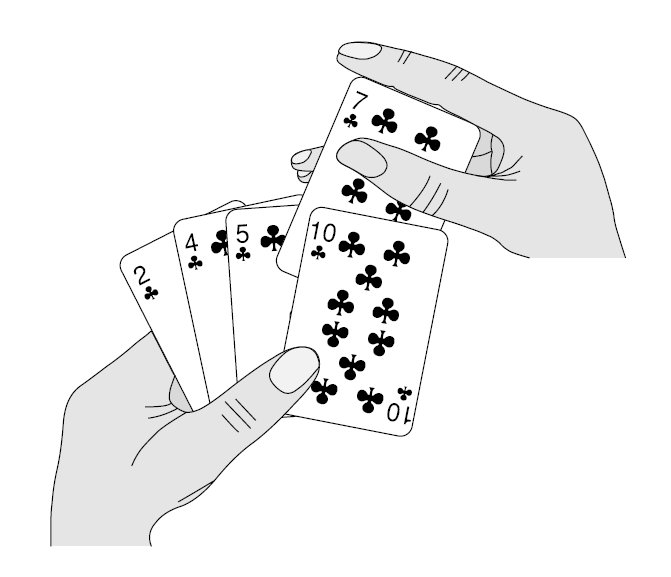
\includegraphics[width = 0.50\textwidth]{figs/poker-insertion-sort} \vspace{-0.30cm}
% 	  \[
% 		\text{Sorting}
% 	  \]
% 	\end{subfigure}
% 	\hfill
% 	\begin{subfigure}[b]{0.45\textwidth}  
% 	  \centering 
% 	  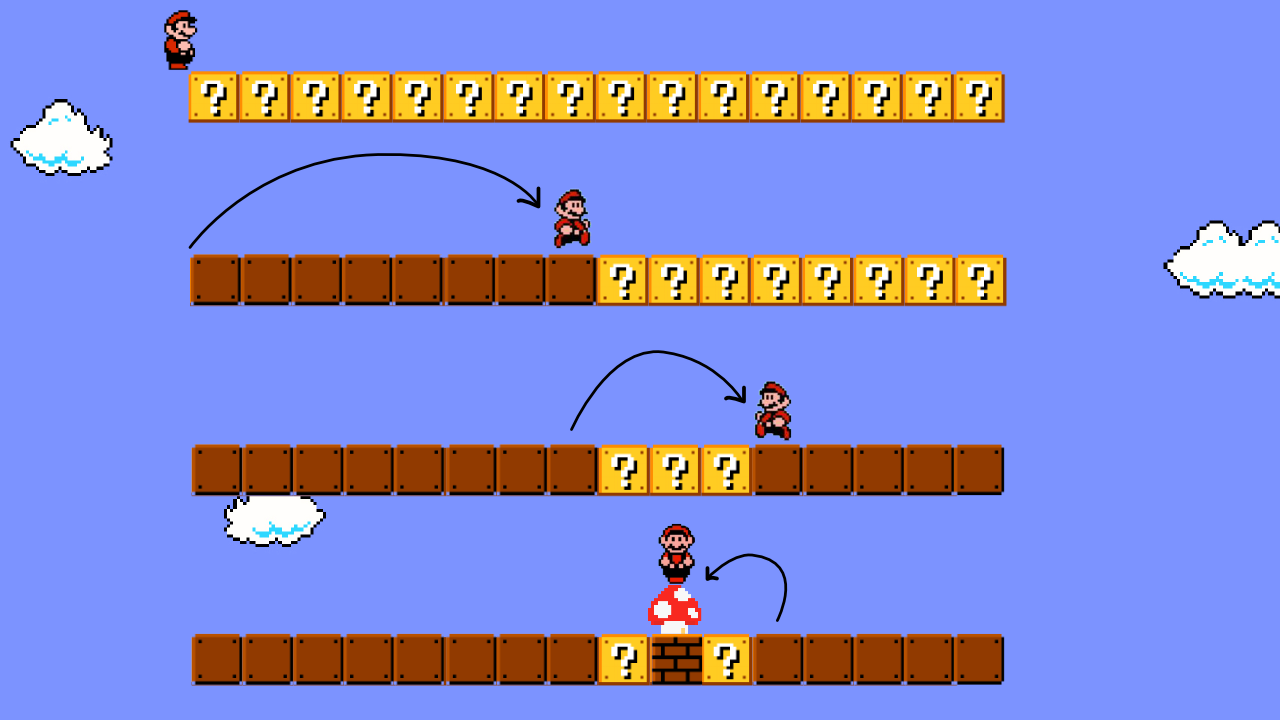
\includegraphics[width = 0.70\textwidth]{figs/binary-stride} \vspace{-0.30cm}
% 	  \[
% 		\text{Searching}
% 	  \]
% 	\end{subfigure}
% 	\vskip\baselineskip
% 	\begin{subfigure}[b]{0.45\textwidth}   
% 	  \centering 
% 	  
\includegraphics[width = 0.60\textwidth]{figs/selection} \vspace{-0.30cm}
% 	  \[
% 		\text{Selection}
% 	  \]
% 	\end{subfigure}
%   \end{figure}
% \end{frame}
%%%%%%%%%%%%%%%
